\section{Руководство пользователя}

\subsection{ Особенности реализации PIC в программе \prognv }

\textbf{Расчетная область и источники частиц.}
Перед началом моделирования нужно определить расчетную область и заселить ее частицами.
Epifc-v0.01 поддерживает расчетную область только прямоугольной формы. 
Что касается генерации частиц - то пока есть возможность задать только один источник.
Кроме того, генерация новых частиц во время работы тоже пока не поддерживается.
\todo{При дискретизации области используется прямоугольная сетка с фиксированным шагом.}
\begin{figure}[h]
  \centering
  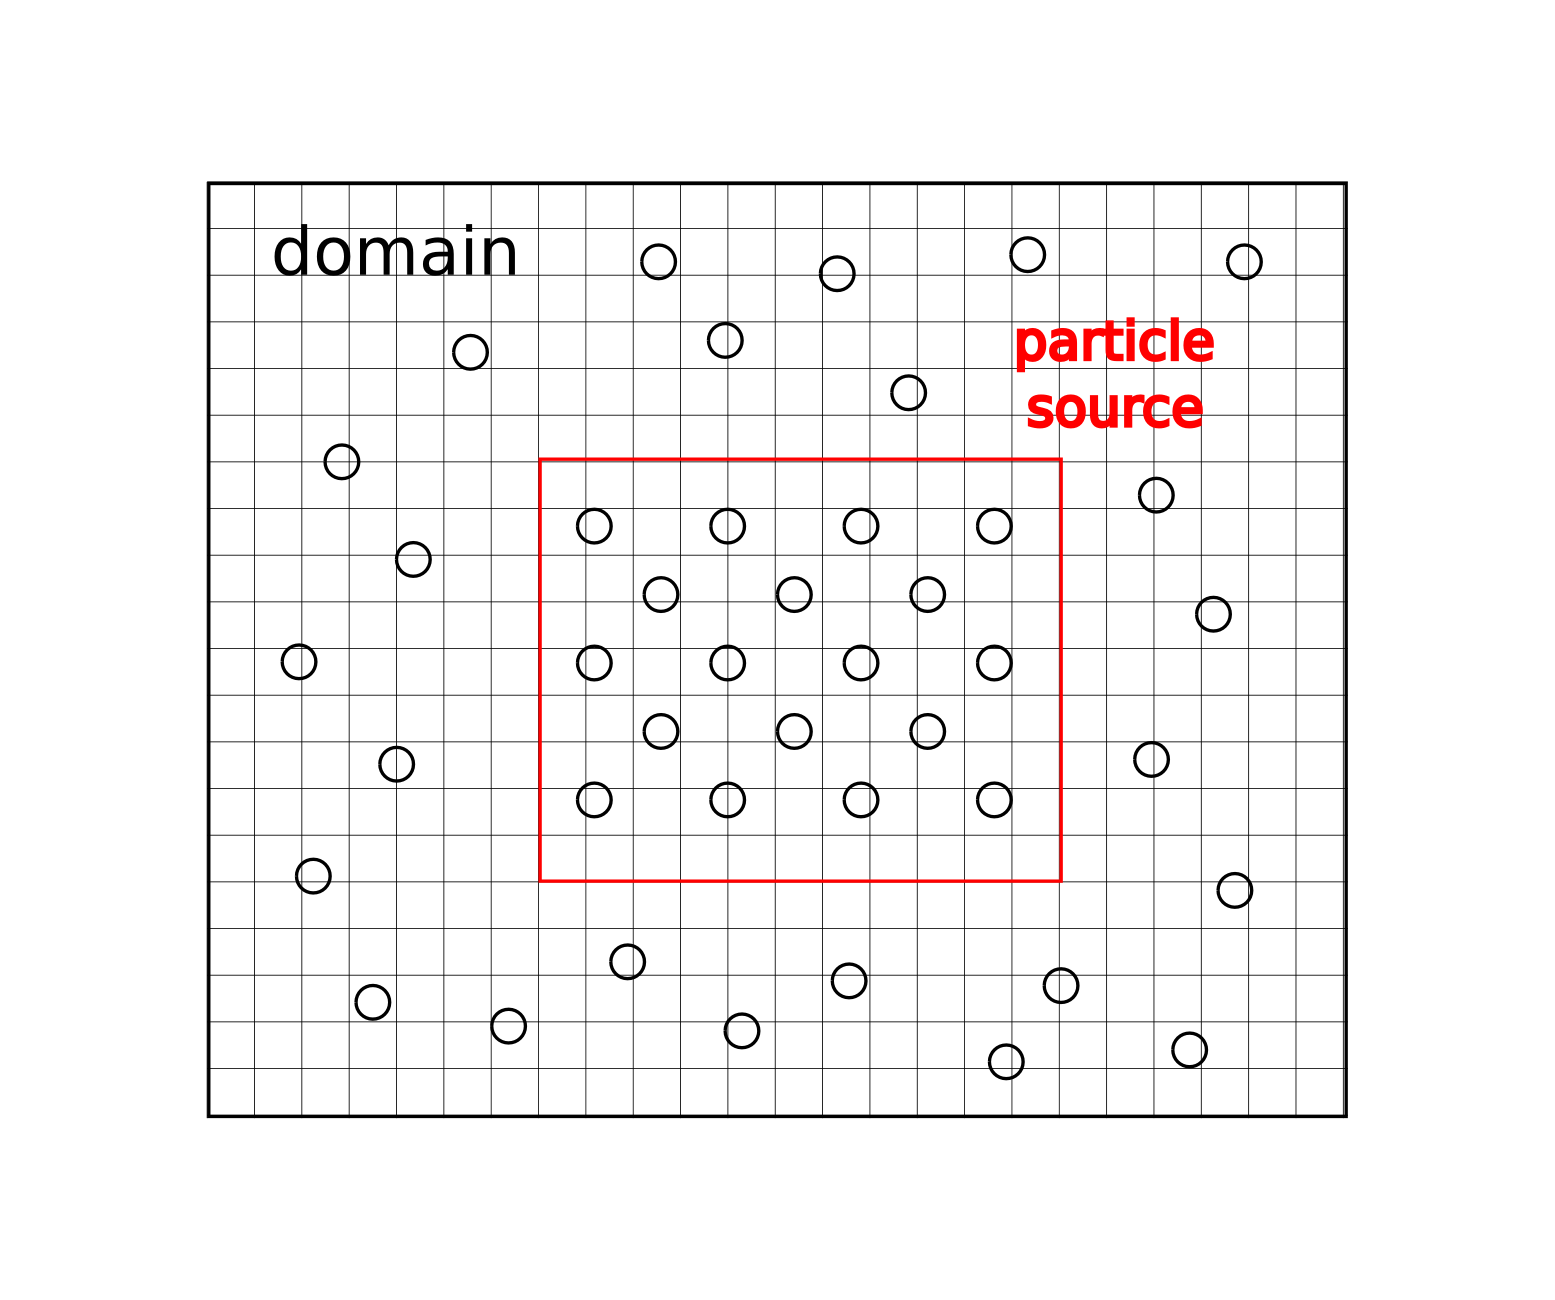
\includegraphics[scale=0.8]{./figs/domain.png}
  \caption{
    Схематичное изображение расчетной области программы.
    \todo{надо его как-то по-аккуратнее сделать}
  }
\end{figure}



\textbf{Связь характеристик макрочастиц с концентрацией реальных частиц и плотностью заряда в области.}
У каждой макрочастицы есть заряд и масса. 
Если концентрация реальных частиц
массой $m_{real}$ и зарядом $q_{real}$
в объеме $V$ равна $n_0\, [1/cm^2]$, 
то масса $m$ и заряд $q$ каждой макрочастицы определяются соотношениями
\begin{gather}
  m = m_{real} \frac{ n_0 V }{ N },
  \quad
  q = q_{real} \frac{ n_0 V }{ N },
\end{gather}
где $N$ - число макрочастиц.
Пользователю необходимо задать массу $m$, заряд $q$ и число макрочастиц $N$
для каждого источника ( см. \ref{sec:config_file} ).

\textbf{Распределение скоростей и координат генерируемых частиц.}
По координатам - равномерно в прямоугольнике.
По импульсам - максвелловское распределение.
\begin{gather}
  f( \vec{p} ) dp = \frac{1}{ 2 \pi m \theta } e^{ - \dfrac{ p_x^2 + p_y^2 }{ 2 m \theta } }
\end{gather}
где $\theta = k T$, $k$ - постоянная Больцмана, $T$ - температура.
В конфигурационном фаиле необходимо задать $\theta$ для каждого источника.


После инициализации частиц запускается алгоритм PIC. 
Вначале происходит интерполяция зарядов макрочастиц на узлы сетки.
Предполагается, что частицы вносят вклад только в ближайшие узлы. 
\todo{Форма частиц - ступенька ( поискать официальное название для этого ).}
\todo{Вставить картинку.}

\todo{Здесь оставить только общие уравнения. Дискретные убрать в раздел с описанием программы.}

Следующий шаг - расчет потенциалов. 
Epicf-v0.01 не поддерживает магнитное поле
и использует только электрическое ( электростатическая модель, ES-PIC ).
Для его нахождения нужно решить уравнение Пуассона:
\begin{gather}
  \Delta \phi = - 4 \pi \rho
\end{gather}
Поддерживаются граничные условия только 1 рода ( на потенциал, а не на поле ).
Они задаются в конфигурационном фаиле.

По найденным значениям потенциала расчитывается значение поля в узлах решетки:
\begin{gather}
  \vec{ E } = - \nabla \phi
\end{gather}

Затем обновляются импульсы и координаты частиц
( при этом происходит обратная интерполяция полей из узлов решетки на частицы ).
\begin{gather}
  \frac{ d \vec{p} }{ d t } = \vec{ F } = q \vec{ E }
  \\
  \frac{ d \vec{r} }{ d t } = \frac{ \vec{p} }{ m }
\end{gather}
Используется схема Leap-frog ( см. след раздел ).
\todo{ дописать пару слов про нее.  }

\textbf{Запись в фаил.}
В конце временного шага можно сохранить результаты расчетов в фаил. 
Записывается вся информация, необходимая для возобновления расчетов.
Детально формат фаила описан в \todo{следующем} разделе. 
Имя выходного фаила генерируется по параметрам в конфигурационном фаиле.
Номер временного шага для записи тоже берется из конфига.




\subsection{ Параметры конфигурационного фаила }
\label{sec:config_file}

Для пользователя, взаимодействие с программой должно ограничиваться изменениями в конфигурационном фаиле.

\todo{Выбор согласованных единиц измерения - задача пользователя. Написать про размерности.}

Описание параметров:

\subsection{ Визуализация результатов }

В комплекте с программой идет скрипт для визуализации результатов.
\todo{переименовать по-проще}
( скрипт на R - см. раздел ``установка'' ).
Лежит в директории plot. Вызывается командой вида
\begin{verbatim}
./rplot_script.r [options] /path_to_output_files/output.dat
\end{verbatim}
где output.dat - выходной фаил, полученный при работе программы.

Пока доступно 3 опции: 
\begin{itemize}
\item -p, --potential - строит значения потенциала в узлах сетки.
\item -d, --density - строит значения плотности заряда в узлах сетки.
\item -P, --particles - рисует частицы и направления их импульсов.
\end{itemize}

Пример:
\begin{verbatim}
./rplot_script.r -pdP ../out/out0001.dat
\end{verbatim}
построит графики для потенциала, плотности заряда и частиц и 
сохранит их в текущей директории в фаилы \texttt{out0001\_potential.png}, 
\texttt{out0001\_density.png} и \texttt{out0001\_particles.png}.
\begin{figure}[h]
  \centering
  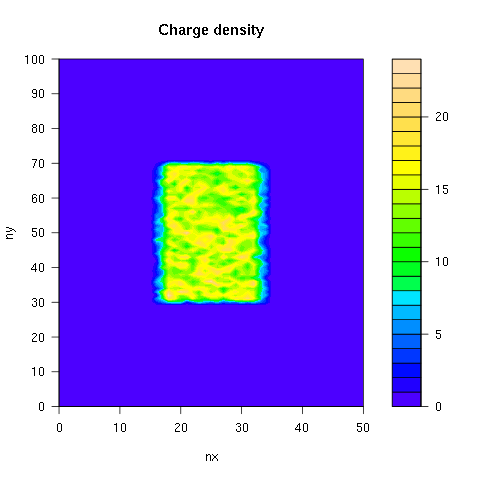
\includegraphics[scale=0.3]{./figs/out0001_density.png}
  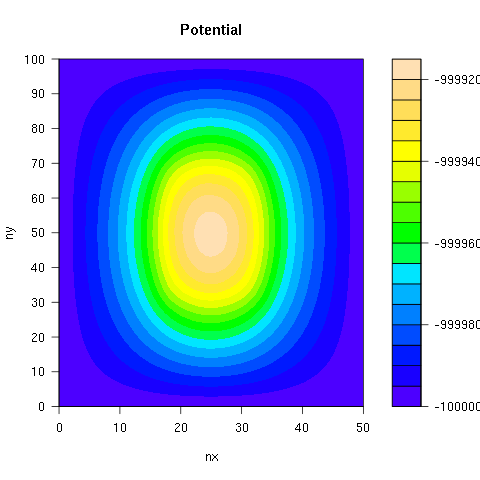
\includegraphics[scale=0.3]{./figs/out0001_potential.png}
  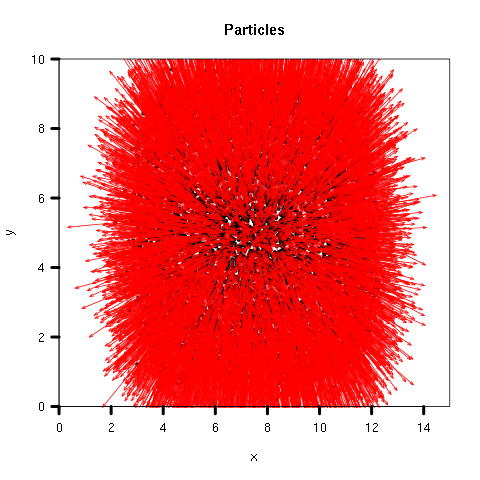
\includegraphics[scale=0.3]{./figs/out0001_particles.png}
  \caption{
    Графики плотности заряда, потенциала и распределения частиц.
  }
\end{figure}

\subsection{ Установка }
Исходные коды Epicf доступны на github. 
Проще всего загрузить их оттуда с помощью команды
\begin{verbatim}
git clone https://github.com/noooway/epicf
\end{verbatim}

Для сборки понадобятся компиляторы gcc и gfortran, а также библиотеки GSL и GLib. \todo{ссылки}.
В большинстве дистрибутивов GNU/Linux эти программы есть в стандартных репозиториях.
На примере Ubuntu, команды для установки имеют вид:
\begin{verbatim}
\todo{apt-install что-то там}
\end{verbatim}
При установке библиотек нужны именно devel-версии.

Когда все необходимое установлено, для сборки Epicf достаточно 
выполнить команду make.
\begin{verbatim}
cd /some-path/epicf
make
\end{verbatim}

Если компиляция прошла успешно, то в директории должен появиться исполняемый фаил epicf.out.
Запустить программу с выбранным конфигурационным фаилом можно с помощью 
\begin{verbatim}
./epicf.out test.conf
\end{verbatim}

В комплекте с программой идет скрипт для визуализации результатов.
Скрипт написан на языке R, поэтому чтобы этим скриптом воспользоваться, нужно установить R:
\begin{verbatim}
\todo{apt-install что-то там}
\end{verbatim}
Также для работы скрипта требуется установить пакет 'optparse' для R.
Это можно сделать, выполнив в командной строке
\begin{verbatim}
R -e "install.packages('optparse', repos='http://cran.us.r-project.org')"
\end{verbatim}
или \texttt{install.packages('optparse')} из консоли R.


%%% Local Variables: 
%%% mode: latex
%%% TeX-master: "major"
%%% End: 
